En adder er en digital krets som adderer to tall.
Vi skal se på 1-bit addere som legger sammen en bit med en annen.
Disse kan igjen settes sammen så man får en n-bit adder.



\paragraph{Halvadder} \mbox{} \\
Addere kommer hovedsaklig i to typer, halv og hel.
Halvaddere har to input og to output.
De to inputene er tallene A og B som skal adderer.
De to ouptupene er summen S og mente C.
Mente er med hvis man får 2 som svar da det ikke kan representeres med 1 bit.
\\\\
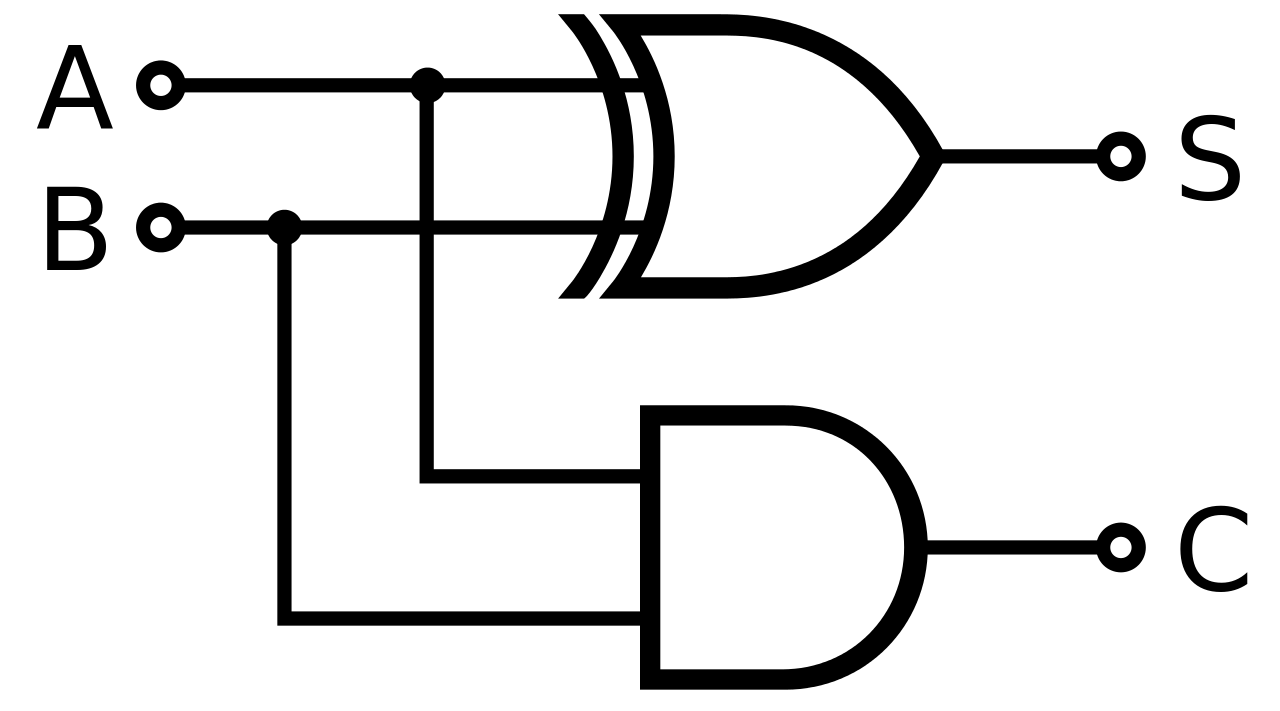
\includegraphics[width=0.5\textwidth]{./img/half-adder}
\\\\
Sannhetstabellen til en halvadder ser ut som følgende
\\\\
\begin{tabular}{c|c|c|c}
  A & B & C & S \\ \hline
  0 & 0 & 0 & 0 \\
  0 & 1 & 0 & 1 \\
  1 & 0 & 0 & 1 \\
  1 & 1 & 1 & 0
\end{tabular}



\paragraph{Heladder} \mbox{} \\
Heladderen har \emph{tre} input, A, B og mente $C_{inn}$ fra forige addisjon.
Output er likt som halvadder: $C_{ut}$ og S
\\\\
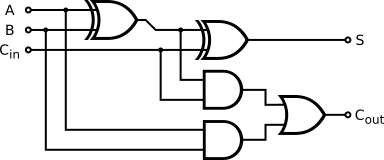
\includegraphics[width=\textwidth]{./img/full-adder}
\\\\
Sannhetstabellen blir litt mer komplisert.
\\\\
\begin{tabular}{c|c|c|c|c}
  A & B & Cin & Cut & S \\ \hline
  0 & 0 & 0 & 0 & 0 \\
  0 & 0 & 1 & 0 & 1 \\
  0 & 1 & 0 & 0 & 1 \\
  0 & 1 & 1 & 1 & 0 \\
  1 & 0 & 0 & 0 & 1 \\
  1 & 0 & 1 & 1 & 0 \\
  1 & 1 & 0 & 1 & 0 \\
  1 & 1 & 1 & 1 & 1
\end{tabular}



\paragraph{n-bit adder} \mbox{} \\
Nå har vi sett på 1-bit addere.
Vi vet hvordan de har A, B og $C_{inn}$ som input og S og $C_{ut}$ som output.
\\\\
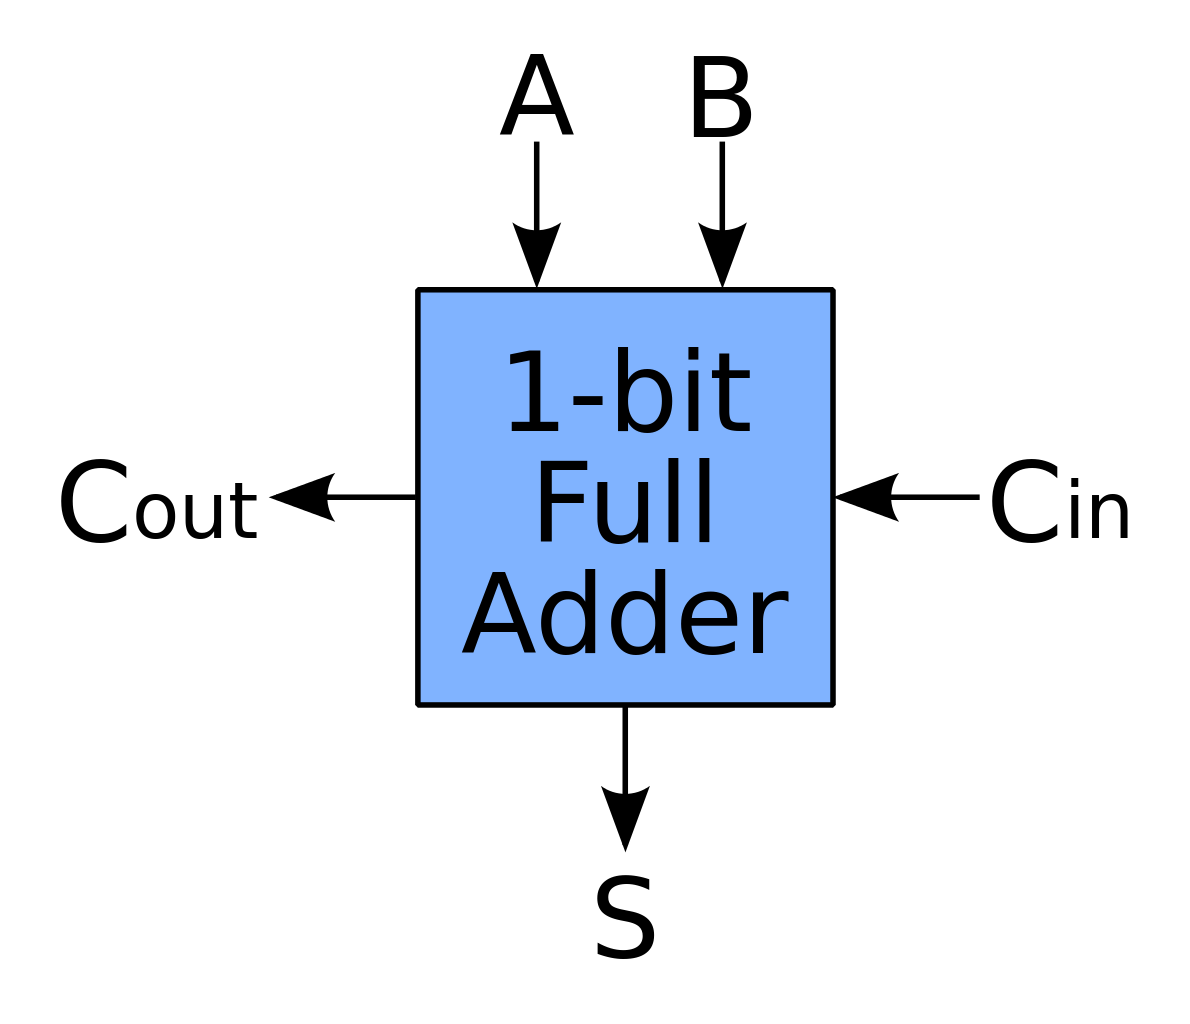
\includegraphics[width=0.5\textwidth]{./img/1bit-adder}
\\\\
Hvis vi vil lage en adder som tar f.eks. 4 bit kan vi simpelthen sette sammen
fire 1-bit addere.
\\\\
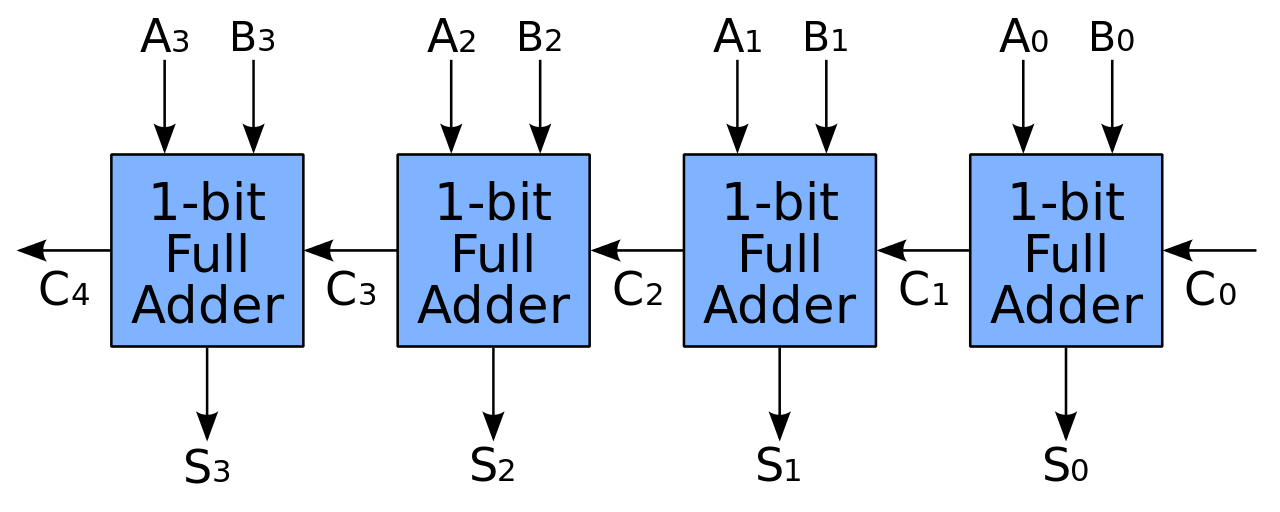
\includegraphics[width=\textwidth]{./img/4bit-adder}
